
%\node[options] (
%\node[options] (
%\coordinate (id) at position;) at position {label};) at position {label};% ------------------------------------------------------------------------
% ------------------------------------------------------------------------
% Modelo UFSC para Trabalhos Academicos (tese de doutorado, dissertação de
% mestrado) utilizando a classe abntex2
%
% Autor: Alisson Lopes Furlani
% 	Modificações:
%	- 27/08/2019: Alisson L. Furlani, add pacote 'glossaries' para listas
%   - 06/11/2019: Luiz-Rafael Santos, modificação para Trabalho de Conclusão de Curso
%   - 10/03/2024: Mateus L. modelo adaptado para Relatório técnico UFPR
% ------------------------------------------------------------------------
% ------------------------------------------------------------------------

\documentclass[
	% -- opções da classe memoir --
	12pt,				% tamanho da fonte
	%openright,			% capítulos começam em pág ímpar (insere página vazia caso preciso)
	oneside,			% para impressão no anverso. Oposto a twoside
	a4paper,			% tamanho do papel. 
	% -- opções da classe abntex2 --
	chapter=TITLE,		% títulos de capítulos convertidos em letras maiúsculas
	section=TITLE,		% títulos de seções convertidos em letras maiúsculas
	%subsection=TITLE,	% títulos de subseções convertidos em letras maiúsculas
	%subsubsection=TITLE,% títulos de subsubseções convertidos em letras maiúsculas
	% -- opções do pacote babel --
	english,			% idioma adicional para hifenização
	%french,				% idioma adicional para hifenização
	%spanish,			% idioma adicional para hifenização
	brazil				% o último idioma é o principal do documento
	]{abntex2}

\usepackage{setup/ufscthesisA4-alf}
\pagestyle{simple}
% ---
% Filtering and Mapping Bibliographies
% ---
% Pacotes de citações
% ---
\usepackage{csquotes}
\usepackage[backend = biber, style = abnt]{biblatex}
% FIXME Se desejar estilo numérico de citações,  comente a linha acima e descomente a linha a seguir.
% \usepackage[backend = biber, style = numeric-comp]{biblatex}

\setlength\bibitemsep{\baselineskip}
\DeclareFieldFormat{url}{Disponível~em:\addspace\url{#1}}
\NewBibliographyString{sineloco}
\NewBibliographyString{sinenomine}
\DefineBibliographyStrings{brazil}{%
	sineloco     = {\mkbibemph{S\adddot l\adddot}},
	sinenomine   = {\mkbibemph{s\adddot n\adddot}},
	andothers    = {\mkbibemph{et\addabbrvspace al\adddot}},
	in			 = {\mkbibemph{In:}}
}

\addbibresource{aftertext/references.bib} % Seus arquivos de referências

% ---
\DeclareSourcemap{
	\maps[datatype=bibtex]{
		% remove fields that are always useless
		\map{
			\step[fieldset=abstract, null]
			\step[fieldset=pagetotal, null]
		}
		% remove URLs for types that are primarily printed
%		\map{
%			\pernottype{software}
%			\pernottype{online}
%			\pernottype{report}
%			\pernottype{techreport}
%			\pernottype{standard}
%			\pernottype{manual}
%			\pernottype{misc}
%			\step[fieldset=url, null]
%			\step[fieldset=urldate, null]
%		}
		\map{
			\pertype{inproceedings}
			% remove mostly redundant conference information
			\step[fieldset=venue, null]
			\step[fieldset=eventdate, null]
			\step[fieldset=eventtitle, null]
			% do not show ISBN for proceedings
			\step[fieldset=isbn, null]
			% Citavi bug
			\step[fieldset=volume, null]
		}
	}
}
% ---

% ---
% Informações de dados para CAPA e FOLHA DE ROSTO
% ---
% FIXME Substituir 'Nome completo do autor' pelo seu nome.
\autor{MATEUS MISCHEL LODI}
% FIXME Substituir 'Título do trabalho' pelo título da trabalho.
\titulo{Meus Boletos}
% FIXME Substituir 'Subtítulo (se houver)' pelo subtítulo da trabalho.  
% Caso não tenha substítulo, comente a linha a seguir.
\subtitulo{um aplicativo web para gestão financeira}
% FIXME Substituir 'XXXXXX' pelo nome do seu
% orientador.
\orientador{Prof. Dr. Razer A. N. R. Montaño}
% FIXME Se for orientado por uma mulher, comente a linha acima e descomente a linha a seguir.
% \orientador[Orientadora]{Nome da orientadora, Dra.}
% FIXME Substituir 'XXXXXX' pelo nome do seu
% coorientador. Caso não tenha coorientador, comente a linha a seguir.
%\coorientador{Prof. XXXXXX, Dr.}
% FIXME Se for coorientado por uma mulher, comente a linha acima e descomente a linha a seguir.
% \coorientador[Coorientadora]{XXXXXX, Dra.}
% FIXME Substituir 'XXXXXX' pelo nome do Coordenador do 
% programa/curso.
\coordenador{Prof. Dr. Jaime Wojciechowski}
% FIXME Se for coordenadora mulher, comente a linha acima e descomente a linha a seguir.
% \coordenador[Coordenadora]{Nome da Coordenadora, Dra.}
% FIXME Substituir '[ano da entrega]' pelo ano (ano) em que seu trabalho foi defendido.
\ano{2024}
% FIXME Substituir '[dia] de [mês] de [ano]' pela data em que ocorreu sua defesa.
\data{21 de abril de 2024}
% FIXME Substituir '[Cidade da defesa]' pela cidade em que ocorreu sua defesa.
\local{CURITIBA}
\instituicaosigla{UFPR}
\instituicao{Universidade Federal do Paraná}
% FIXME Substituir 'Dissertação/Tese' pelo tipo de trabalho (Tese, Dissertação). 
\tipotrabalho{Relatório Técnico}
% FIXME Substituir '[licenciado/bacharel] em [nome do título obtido]' pela grau adequado.
\formacao{Pós-graduação lato sensu}
% FIXME Substituir '[licenciado/bacharel]' pelo nivel adequado.
\nivel{Especialista}
% FIXME Substituir 'Curso de Graduação em [XXXXXXXX]' pela curso adequado.
\programa{Curso de Especialização em Desenvolvimento Ágil de Software}
% FIXME Substituir 'Campus XXXXXX ou Centro de XXXXXX' pelo campus ou centro adequado.
\centro{Setor de Educação Profissional e Tecnológica}
\preambulo
{%
\imprimirtipotrabalho~do~\imprimirprograma~do~\imprimircentro~da~\imprimirinstituicao
}
% ---

% ---
% Configurações de aparência do PDF final
% ---
% alterando o aspecto da cor azul
\definecolor{blue}{RGB}{41,5,195}
% informações do PDF
\makeatletter
\hypersetup{
     	%pagebackref=true,
		pdftitle={\@title}, 
		pdfauthor={\@author},
    	pdfsubject={\imprimirpreambulo},
	    pdfcreator={LaTeX with abnTeX2},
		pdfkeywords={ufsc, latex, abntex2}, 
		colorlinks=true,       		% false: boxed links; true: colored links
    	linkcolor=black,%blue,          	% color of internal links
    	citecolor=black,%blue,        		% color of links to bibliography
    	filecolor=black,%magenta,      		% color of file links
		urlcolor=black,%blue,
		bookmarksdepth=4
}
\makeatother
% ---

% ---
% compila a lista de abreviaturas e siglas e a lista de símbolos
% ---

% Declaração das siglas
\siglalista{ABNT}{Associação Brasileira de Normas Técnicas}

% Declaração dos simbolos
\simbololista{C}{\ensuremath{C}}{Circunferência de um círculo}
\simbololista{pi}{\ensuremath{\pi}}{Número pi} 
\simbololista{r}{\ensuremath{r}}{Raio de um círculo}
\simbololista{A}{\ensuremath{A}}{Área de um círculo}

% compila a lista de abreviaturas e siglas e a lista de símbolos
\makenoidxglossaries 

% ---

% ---
% compila o indice
% ---
\makeindex
% ---

% ----
% Início do documento
% ----
\begin{document}

% Seleciona o idioma do documento (conforme pacotes do babel)
%\selectlanguage{english}
\selectlanguage{brazil}

% Retira espaço extra obsoleto entre as frases.
\frenchspacing 

% Espaçamento 1.5 entre linhas
\OnehalfSpacing

% Corrige justificação
%\sloppy

% ----------------------------------------------------------
% ELEMENTOS PRÉ-TEXTUAIS
% ----------------------------------------------------------
% \pretextual %a macro \pretextual é acionado automaticamente no início de \begin{document}
% ---
% Capa, folha de rosto, ficha bibliografica, errata, folha de apróvação
% Dedicatória, agradecimentos, epígrafe, resumos, listas
% ---
% ---
% Capa
% ---
\imprimircapa
% ---

% ---
% Folha de rosto
% (o * indica que haverá a ficha bibliográfica)
% ---
\imprimirfolhaderosto*
% ---

% ---
% Inserir a ficha bibliografica
% ---
% http://ficha.bu.ufsc.br/
%\begin{fichacatalografica}
%	\includepdf{beforetext/Ficha_Catalografica.pdf}
%\end{fichacatalografica}
% ---

% ---
% Inserir folha de aprovação
% ---

%\begin{folhadeaprovacao}
%	\OnehalfSpacing
%	\centering
%	\imprimirautor\\%
%	\vspace*{10pt}		
%	\textbf{\imprimirtitulo}%
%	\ifnotempty{\imprimirsubtitulo}{:~\imprimirsubtitulo}\\%
%	%		\vspace*{31.5pt}%3\baselineskip
%	\vspace*{\baselineskip}
%	%\begin{minipage}{\textwidth}
%	% ~do~\imprimirprograma~do~\imprimircentro~da~\imprimirinstituicao~para~a~obtenção~do~título~de~\imprimirformacao.
%	Este~\imprimirtipotrabalho~foi julgado adequado para obtenção do Título de “\imprimirformacao” e aprovado em sua forma final pelo~\imprimirprograma. \\
%		\vspace*{\baselineskip}
%	\imprimirlocal, \imprimirdata. \\
%	\vspace*{2\baselineskip}
%	\assinatura{\OnehalfSpacing\imprimircoordenador \\ \imprimircoordenadorRotulo~do Curso}
%	\vspace*{2\baselineskip}
%	\textbf{Banca Examinadora:} \\
%	\vspace*{\baselineskip}
%	\assinatura{\OnehalfSpacing\imprimirorientador \\ \imprimirorientadorRotulo}
%	%\end{minipage}%
%	\vspace*{\baselineskip}
%	\assinatura{Prof.(a) xxxx, Dr(a).\\
%	Avaliador(a) \\
%	Instituição xxxx}
%
%	\vspace*{\baselineskip}
%	\assinatura{Prof.(a) xxxx, Dr(a).\\
%	Avaliador(a) \\
%	Instituição xxxx}


%\end{folhadeaprovacao}
% ---

% ---
% Dedicatória
% ---
%\begin{dedicatoria}
%	\vspace*{\fill}
%	\noindent
%	\begin{adjustwidth*}{}{5.5cm}     
%		Este trabalho é dedicado aos meus colegas de classe e aos meus queridos pais.
%	\end{adjustwidth*}
%\end{dedicatoria}
% ---

% ---
% Agradecimentos
% ---
%\begin{agradecimentos}
%	Inserir os agradecimentos aos colaboradores à execução do trabalho. 
	
%	Xxxxxxxxxxxxxxxxxxxxxxxxxxxxxxxxxxxxxxxxxxxxxxxxxxxxxxxxxxxxxxxxxxxxxx. 
%\end{agradecimentos}
% ---

% ---
% Epígrafe
% ---
%\begin{epigrafe}
%	\vspace*{\fill}
%	\begin{flushright}
%		\textit{``Texto da Epígrafe.\\
%			Citação relativa ao tema do trabalho.\\
%			É opcional. A epígrafe pode também aparecer\\
%			na abertura de cada seção ou capítulo.\\
%			Deve ser elaborada de acordo com a NBR 10520.''\\
%			(Autor da epígrafe, ano)}
%	\end{flushright}
%\end{epigrafe}
% ---

% ---
% RESUMOS
% ---

% resumo em português
\setlength{\absparsep}{18pt} % ajusta o espaçamento dos parágrafos do resumo
\begin{resumo}
	\SingleSpacing
    O endividamento tem sido uma questão crescente para as famílias brasileiras, com uma grande proporção delas enfrentando algum tipo de dívida. A inadimplência, liderada principalmente pelo uso de cartões de crédito, reflete desafios tanto macro quanto microeconômicos, como desemprego e falta de planejamento financeiro. Além disso, o impacto psicológico da inadimplência é significativo, afetando negativamente o bem-estar mental e físico das pessoas. Em resposta a esses desafios, foram criadas diversas estratégias para promover uma melhor compreensão e gestão das finanças pessoais. Essas iniciativas já resultaram em várias ações voltadas para a educação financeira. Visando aprofundar os esforços dessas iniciativas, propõe-se o desenvolvimento de uma aplicação web dedicada à gestão financeira. Essa ferramenta visa facilitar o controle financeiro diário, oferecendo recursos de planejamento e uma plataforma para aprendizado contínuo. O objetivo é melhorar a saúde financeira dos usuários, tornando a educação financeira mais acessível e prática através de soluções tecnológicas.
	
	\textbf{Palavras-chave}: Aplicativo. inadimplência. Financeiro. Contas
\end{resumo}

% resumo em inglês
\begin{resumo}[Abstract]
	\SingleSpacing
	\begin{otherlanguage*}{english}
		Debt has been an increasing issue for Brazilian families, with a large proportion of them facing some type of debt. Delinquency, primarily led by the use of credit cards, reflects both macro and microeconomic challenges, such as unemployment and lack of financial planning. Moreover, the psychological impact of delinquency is significant, negatively affecting people's mental and physical well-being. In response to these challenges, various strategies have been created to promote a better understanding and management of personal finances. These initiatives have already resulted in several actions aimed at financial education. To further the efforts of these initiatives, the development of a web application dedicated to financial management is proposed. This tool aims to facilitate daily financial control, offering planning resources and a platform for continuous learning. The goal is to improve the financial health of users, making financial education more accessible and practical through technological solutions.
		
		\textbf{Keywords}: Apps. Debts. Finance. Fees.
	\end{otherlanguage*}
\end{resumo}

%% resumo em francês 
%\begin{resumo}[Résumé]
% \begin{otherlanguage*}{french}
%    Il s'agit d'un résumé en français.
% 
%   \textbf{Mots-clés}: latex. abntex. publication de textes.
% \end{otherlanguage*}
%\end{resumo}
%
%% resumo em espanhol
%\begin{resumo}[Resumen]
% \begin{otherlanguage*}{spanish}
%   Este es el resumen en español.
%  
%   \textbf{Palabras clave}: latex. abntex. publicación de textos.
% \end{otherlanguage*}
%\end{resumo}
%% ---

%{%hidelinks
%	\hypersetup{hidelinks}
	% ---
	% inserir lista de ilustrações
	% ---
	\pdfbookmark[0]{\listfigurename}{lof}
	\listoffigures*
	\cleardoublepage
	% ---
	
	% ---
	% inserir lista de quadros
	% ---
	%\pdfbookmark[0]{\listofquadrosname}{loq}
	%\listofquadros*
	%\cleardoublepage
	% ---
	
	% ---
	% inserir lista de tabelas
	% ---
	\pdfbookmark[0]{\listtablename}{lot}
	\listoftables*
	\cleardoublepage
	% ---
	
	% ---
	% inserir lista de abreviaturas e siglas (devem ser declarados no preambulo)
	% ---
%	\imprimirlistadesiglas
	% ---
	
	% ---
	% inserir lista de símbolos (devem ser declarados no preambulo)
	% ---
%	\imprimirlistadesimbolos
	% ---
	
	% ---
	% inserir o sumario
	% ---
{
	\pdfbookmark[0]{\contentsname}{toc}
	\tableofcontents*
	\cleardoublepage
}	
%}%hidelinks
% ---
% ---

% ----------------------------------------------------------
% ELEMENTOS TEXTUAIS
% ----------------------------------------------------------
\textual

% ---
% 1 - Visão geral do Projeto
% ---
% ----------------------------------------------------------
\chapter{Visão Geral do Projeto}
% ----------------------------------------------------------



% ----------------------------------------------------------
\section{Contextualização}
% ----------------------------------------------------------

O endividamento de famílias brasileiras atingiu 78,1\% em março de 2024 de acordo com CNC (2024). Isso representa que aproximadamente 8 a cada 10 famílias possuem algum tipo de dívida, seja ela atrasada ou não. É considerada inadimplente a parcela da população que possui dívidas atrasadas, ou seja, deixou de pagar uma dívida no vencimento ou o não cumprimento de um contrato ou clausula de contrato (Sehn et Carlini Junior, 2007).

A parcela inadimplente das famílias brasileiras representou 28,5\% em março de 2024 segundo CNDL (2024). O alto nível de inadimplência retrata não apenas as dificuldades econômicas enfrentadas num pais, mas partindo de um olhar microeconômico  situações comuns como desemprego, despesas inesperadas, falta de planejamento financeiro, compras para terceiros e ausência de educação financeira (SPC,2024).

De acordo com  Serasa (2024), as principais dividas por segmento em fevereiro de 2024 são: Cartão de Crédito com 29,27\%, contas básicas como água e luz são 22,67\%, financeiras com 17,17\% e varejo com 10,99\%. O fato do cartão de crédito ser a principal forma de inadimplência, pode ser interpretado que ele seja entendido como uma extensão de renda mensal das pessoas, no entanto, o que acontece é um empréstimo pré-estabelecido a ser pago posteriormente.

Os impactos sofridos pelo endividamento vão além do financeiro, segundo Serasa (2022) aponta que 83\% dos devedores têm dificuldade para dormir, 78\% dos entrevistados têm surtos de pensamentos negativos devido em relação as inadimplências e 61\% têm crises de ansiedade ao pensar na dívida. Os dados apresentados ressaltam que possuir uma vida financeira saudável contribui não só com saúde mental mas com a satisfação das necessidades fisiológicas do cidadão: moradia e alimentação, isso vai de encontro com Araújo e Souza (2012), cujas ideias, expressam que com um planejamento melhor da vida financeira e menos envolvimento com necessidade de crédito torna a saúde financeira mais fundamentada.  

 Por conta da importância dada à educação financeira, foi criada em 2010 a Estratégia Nacional de Educação Financeira (ENEF), cujo principal objetivo é promover a educação financeira e previdenciária de acordo com MEC(2024). A ENEF é governamental e possui mais de 1300 iniciativas relacionadas a educação financeira (CUNHA, 2022). Diante desse cenário, surge a necessidade de ferramentas práticas que auxiliem os indivíduos a aplicarem os conhecimentos adquiridos em sua rotina financeira. 

Nesse contexto, o desenvolvimento de uma aplicação web dedicada à gestão financeira pode representar um passo significativo. Esta aplicação não apenas facilitaria o dia a dia dos usuários ao oferecer funcionalidades de controle e planejamento financeiro, mas também serviria como uma plataforma interativa de aprendizado contínuo em finanças, alinhando-se assim aos objetivos da ENEF de fomentar a educação financeira de maneira acessível e prática.

Diante dos problemas e oportunidades apresentadas, o principal objetivo deste trabalho é desenvolver uma aplicação web, que auxilie o usuário com a gestão financeira, permitindo e a visualização de suas finanças de forma simples.


% ----------------------------------------------------------
\section{Descrição do projeto do Produto}
% ----------------------------------------------------------


Este projeto visa desenvolver um aplicativo móvel focado na gestão financeira individual, oferecendo aos usuários a capacidade de gerir o próprio orçamento, além de documentar e categorizar receitas e gastos para uma melhor análise e visualização.

O aplicativo Web inclui funcionalidades como a geração de gráficos de despesas segregados por categoria e a exibição do saldo mensal total, facilitando aos usuários uma compreensão mais clara de suas finanças. Esses recursos visam auxiliar na tomada de decisões financeiras mais informadas e baseadas em dados concretos.

Em síntese, a aplicação Web é projetada para proporcionar aos usuários uma gestão financeira mais efetiva. Ao facilitar o registro organizado de receitas e despesas, categorizando-as e apresentando insights valiosos sobre o comportamento de gastos e rendimentos ao longo de diversos intervalos temporais, os usuários ganham um controle aprimorado sobre sua saúde financeira.

% ----------------------------------------------------------
\section{Funcionalidades}
% ----------------------------------------------------------

\begin{itemize}
    \item Usuário gera um cadastro para si mesmo, assim como uma senha;
    \item Usuário cria categorias para entrada ou saida de dinheiro;
    \item Usuário cria orçamentos mensais;
    \item Usuário criar filtros para seus lançamentos
\end{itemize}

% ----------------------------------------------------------
\section{Tecnologias Usadas}
% ----------------------------------------------------------

As escolhas das tecnologias foram baseadas em 3 fatores: relevância no mercado de trabalho, documentação extensiva disponível na internet, curva de aprendizagem. Com a escolha da ferramentas, a arquitetura da aplicação pode ser definida e é mostrada na figura \ref{fig:process_macro}: 



\begin{figure}[htb]
	\caption{\label{fig:process_macro}Processo macro.}
	\begin{center}
		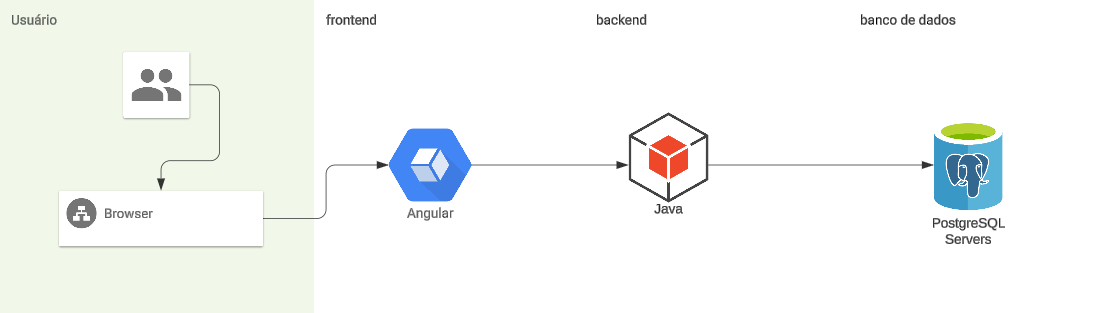
\includegraphics[scale=0.5]{images/processoMacro.png}
	\end{center}
	\fonte{Autor (2024)}
\end{figure}

Como pode ser visto na figura \ref{fig:process_macro} as principais ferramentas são definidas em:

\begin{itemize}
    \item Frontend: Interface de usuário baseada na linguagem Angular;
    \item Backend: API REST programada em Java, com SpringBoot;
    \item Banco de dados: Banco de dados relacional PostgreSQL.
\end{itemize}

\subsection{Java}

 Java é uma linguagem de programação orientada a objetos que é conhecida por sua portabilidade entre plataformas, o que significa que programas escritos em Java podem ser executados em qualquer dispositivo que possua a máquina virtual Java (JVM). Amplamente utilizada para o desenvolvimento de aplicações empresariais, sistemas de gerenciamento de bancos de dados, aplicativos móveis e sistemas embarcados, Java é apreciada por sua robustez, segurança e escalabilidade.

\subsection{SpringBoot}

Spring Boot é um projeto da vasta plataforma Spring que facilita o processo de configuração e publicação de aplicações baseadas em Spring. Esta ferramenta oferece uma maneira rápida e altamente eficaz de desenvolver aplicações stand-alone que podem ser executadas em produção quase que imediatamente. Spring Boot é notável por simplificar o processo de desenvolvimento, oferecendo configurações automáticas e um vasto conjunto de funcionalidades que aceleram o desenvolvimento de aplicações Spring.

\subsection{Angular}

Angular é um framework de desenvolvimento para a construção de aplicações web dinâmicas. Utilizando TypeScript como linguagem principal, Angular oferece aos desenvolvedores uma arquitetura robusta para a construção de interfaces de usuário ricas e interativas, com recursos como data-binding bidirecional, injeção de dependência e um sistema de rotas extensivo. Angular é especialmente benéfico para projetos que necessitam de uma estrutura organizada e escalável para aplicações de página única (SPA).

\subsection{PostgreSQL}

PostgreSQL é um sistema de gerenciamento de banco de dados relacional avançado, conhecido por sua robustez e conformidade com os padrões SQL. É uma solução de código aberto amplamente utilizada em todo o mundo por sua capacidade de lidar com grandes volumes de dados, extensa capacidade de personalização e suporte a uma vasta gama de tipos de dados, incluindo tipos geométricos e de rede. PostgreSQL se destaca pela sua arquitetura sofisticada que suporta transações, subconsultas, triggers, views e procedimentos armazenados, tornando-o uma escolha ideal para aplicações complexas e sistemas que exigem alta integridade de dados. Além disso, é altamente extensível, permitindo aos desenvolvedores adicionar novas funções, tipos de dados e até mesmo escrever código em diferentes linguagens de programação diretamente no banco de dados. Esta flexibilidade faz do PostgreSQL uma opção poderosa tanto para pequenas aplicações quanto para grandes empresas que necessitam de um sistema de banco de dados confiável e escalável.

\subsection{Notion}

Notion é uma aplicação versátil de organização e produtividade que permite aos usuários criar, compartilhar e gerenciar notas, tarefas, bancos de dados e wikis, tudo em um único espaço. A plataforma é altamente flexível, permitindo uma personalização extensa para se adequar a diferentes necessidades de fluxos de trabalho, seja para uso pessoal, acadêmico ou profissional. O Notion se destaca por sua interface de usuário intuitiva e capacidades de colaboração em tempo real. 

\subsection{Lucidchart}

Lucidchart é uma plataforma online de diagramação e visualização de dados que facilita a criação de diagramas complexos usados em diversas áreas, como engenharia de software, design de rede e processos de negócios. Com uma interface drag-and-drop, Lucidchart permite aos usuários colaborar em tempo real, tornando-o uma ferramenta ideal para equipes remotas e projetos que exigem planejamento visual e organização de ideias complexas.


\subsection{Hardware}

O hardware utilizado no desenvolvimento e testes foi um PC desktop com as configurações:

\begin{itemize}
    \item Processador: AMD Ryzen 5 5500;
    \item Placa mãe: MSI B550M PRO-VDH
    \item Memória RAM: 16 GB
    \item Memoria ROM: 1TB SSD
\end{itemize}

\nocite{cnc2024}
\nocite{SPCetCDNL}
\nocite{serasa}
\nocite{serasa2022}
\nocite{Sehn}
\nocite{araujo}
\nocite{MEC}
\nocite{larrisaENEF}
% ---

% 2 - Desenho de casos de Uso
% ---
% ----------------------------------------------------------
\chapter{DESENHO DO PROCESSO MACRO}\label{cap:macro}


\section{Desenho do processo da aplicação}



\begin{figure}[htb]
	\caption{\label{fig:mainProcess}Processo principal da aplicação .}
	\begin{center}
		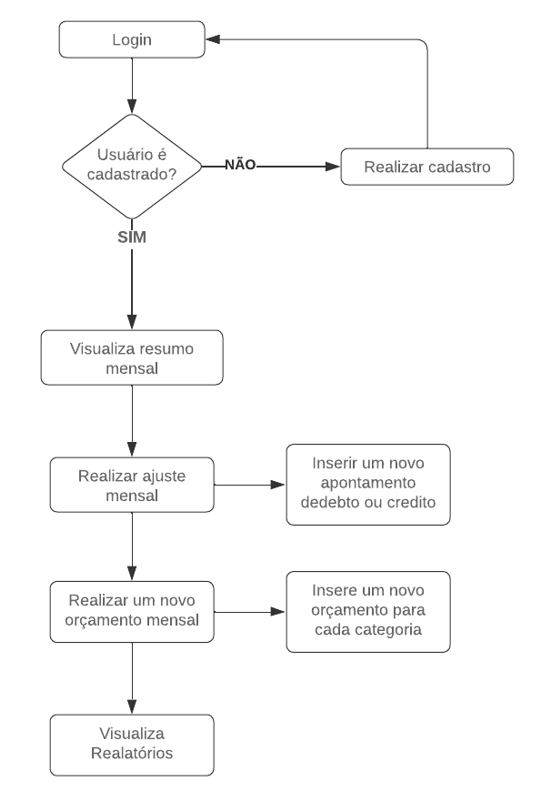
\includegraphics[scale=0.5]{images/ProcessoAplicacao.png}
	\end{center}
	\fonte{Autor (2024)}
\end{figure}







% ---

% 3 - Diagrama de casos de uso
% ---
% ----------------------------------------------------------
\chapter{DIAGRAMA DE CASOS DE USO}
% ----------------------------------------------------------


\begin{figure}[htb]
	\caption{\label{fig:useCase}Diagrama de caso de uso para MeusBoleto.}
	\begin{center}
		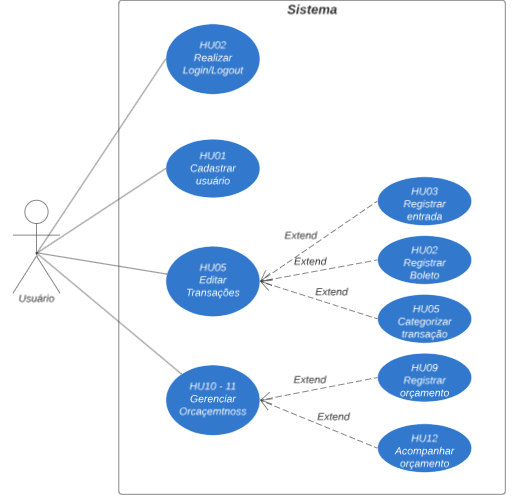
\includegraphics[scale=1]{images/UseCase.png}
	\end{center}
	\fonte{Autor (2024)}
\end{figure}

% ---

% 4 - Diagrama de sequência
% ---
%\phantompart
% ----------------------------------------------------------
\chapter{HISTÓRIAS DE USUÁRIO}
% ----------------------------------------------------------

\begin{itemize}
    \item HU01 Cadastro do Usuário
    \item HU02 Realizar Login/Logout
    \item HU03 Criar Boletos
    \item HU04 Deletar Boletos
    \item HU05 Editar Boletos
    \item HU06 Criar fonte de Renda
    \item HU07 Deletar fonte de Renda
    \item HU08 Editar fonte de Renda
    \item HU09 Criar Orçamento
    \item HU10 Deletar Orçamento
    \item HU11 Editar Orçamento
    \item HU12 Visualizar Resumo

\end{itemize}

\section{Detalhamento das histórias}

\subsection{HU01 Cadastro do Usuário}

Sendo um novo usuario da aplicação, quero me cadastrar na aplicacao, para que consiga usar a aplicação com segurança.

\begin{figure}[htb]
	\caption{\label{fig:hu01}Cadastro de usuário.}
	\begin{center}
		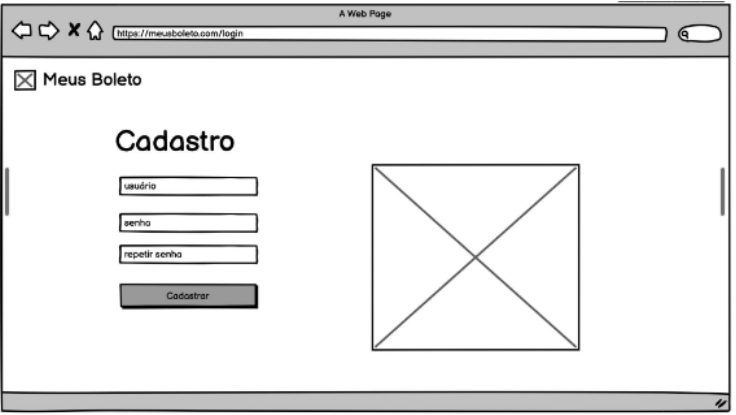
\includegraphics[scale=0.5]{images/Cadastro.png}
	\end{center}
	\fonte{Autor (2024)}
\end{figure}

\textbf{CRITÉRIOS DE ACEITAÇÃO}

\begin{enumerate}
    \item Deve permitir o usuário cadastrar no sistema informando um apelido e senha.
    \item Não deve permitir campos vazios
    \item Não deve permitir senha com menos de 12 caracteres
    \item Deve validar se usuário já existe
    \item Deve validar se as senhas são iguais
\end{enumerate}

\textbf{CRITÉRIOS DE ACEITAÇÃO - DETALHAMENTO}

\textbf{Critério de contexto (Válido como premissa para todos os critérios):}

\begin{itemize}
    \item[\textbf{Dado que}] não tenho acesso a aplicação
    \item[\textbf{E}] estou na tela de cadastro
\end{itemize}


\begin{itemize}
    \item[] \textbf{1. Deve permitir o usuário cadastrar no sistema informando um apelido e senha}

    \begin{itemize}
        \item[\textbf{Dado que}] preenchi o campo senha
        \item[\textbf{E}] o campo do 'repetir senha'.
        \item[\textbf{E}] o campo do usuário.
        \item[\textbf{Quando}] pressiono o botão ``Cadastrar''
        \item[\textbf{Então}] o sistema deve realizar o registro dos meus dados
    \end{itemize}

    \item[] \textbf{2. Não deve permitir campos vazios}
    
    \begin{itemize}
        \item[\textbf{Dado que}] não preenchi algum campo da tela
        \item[\textbf{Quando}] pressiono o botão ``Cadastrar''
        \item[\textbf{Então}] o sistema deve apresentar um erro me informando (R1)
    \end{itemize}

     \item[] \textbf{3. Não deve permitir senha com menos de 12 caracteres}
    
    \begin{itemize}
        \item[\textbf{Dado que}] preenchi o campo da senha com menos de 12 caracteres
        \item[\textbf{E}] e o campo de repetir com a mesma senha
        \item[\textbf{Quando}] pressiono o botão ``Cadastrar''
        \item[\textbf{Então}] o sistema deve apresentar um erro dizendo ao usuário sobre o tamanho das senhas (R1)
    \end{itemize}

     \item[] \textbf{4. Deve validar se usuário já existe}
    
    \begin{itemize}
        \item[\textbf{Dado que}] preenchi o campo de usuário
        \item[\textbf{E}] o campo das senhas corretamente
        \item[\textbf{Quando}] pressiono o botão ``Cadastrar''
        \item[\textbf{Então}] o sistema deve validar se o usuário já existe no sistema se sim, deve apresentar o erro ao usuário (R1)
    \end{itemize}

     \item[] \textbf{5. Deve validar se as senhas são iguais}
    
    \begin{itemize}
        \item[\textbf{Dado que}] preenchi o campo da senha com uma senha
        \item[\textbf{E}] a repetição da senha com outra
        \item[\textbf{Quando}] pressiono o botão ``Cadastrar''
        \item[\textbf{Então}] o sistema deve verificar se as senhas são iguais e aprentar a mensagem de erro apropriada.(R1)
    \end{itemize}

  
\end{itemize}

\textbf{REGRAS DE NEGÓCIO DA HISTÓRIA:}

    R1 - Campos inconsistentes

    \begin{table}[htb]
        \caption{Tabela de inconsistências de cadastro}
        \centering
        \begin{tabular}{|c|c|}
        \hline
          \textbf{Incosistência}   &  \textbf{Mensagem} \\
        \hline
        Campos vazios   & "O campo não deve estar vazio!" \\
        \hline
        Senha não permitida   & "A senha deve possuir 12 ou mais caracteres!" \\
        \hline
        Senhas não conferem   & "As senhas devem ser iguais" \\
        \hline
        \end{tabular}
        \fonte{Autor (2024)}
        \label{tab:tabela_cadastro}
    \end{table}
    
\subsection{HU02 Realizar Login/Logout}

Sendo um usuario da aplicação, quero logar na aplicação para que consiga acessar meus dados.

\begin{figure}[htb]
	\caption{\label{fig:hu02}Login do usuário.}
	\begin{center}
		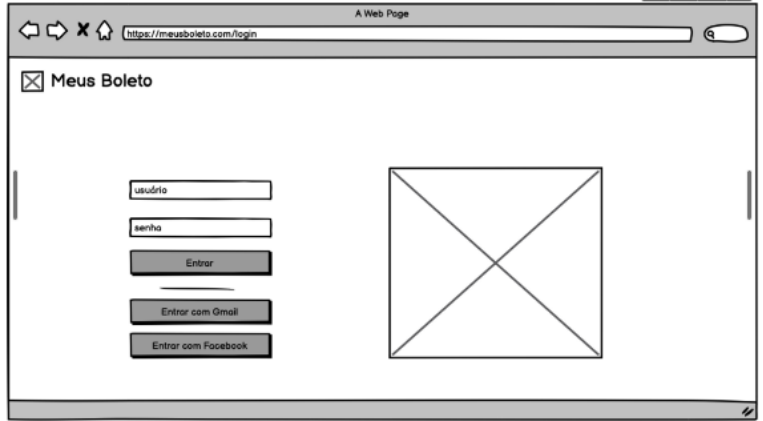
\includegraphics[scale=0.5]{images/Login.png}
	\end{center}
	\fonte{Autor (2024)}
\end{figure}


\textbf{CRITÉRIOS DE ACEITAÇÃO}

\begin{enumerate}
    \item Deve permitir o usuário entrar no sistema.
    \item Deve validar usuário se senha
    \item Não deve permitir acesse se dados estivem incorretos
\end{enumerate}

\textbf{CRITÉRIOS DE ACEITAÇÃO - DETALHAMENTO}

\textbf{Critério de contexto (Válido como premissa para todos os critérios):}

\begin{itemize}
    \item[\textbf{Dado que}] eu tenho um nome de usuário e senha da aplicação
    \item[\textbf{E}] estou na tela de login
\end{itemize}


\begin{itemize}
    \item[] \textbf{1. Deve permitir o usuário entrar no sistema.}

    \begin{itemize}
        \item[\textbf{Dado que}] preenchi o campo 'usuário'
        \item[\textbf{E}] o campo do 'senha'.
        \item[\textbf{Quando}] pressiono o botão ``Entrar''
        \item[\textbf{Então}] o sistema deve permitir a minha estrada no sistema levando-o a tela inicial.
    \end{itemize}

    \item[] \textbf{2. Deve validar usuário se senha.}

    \begin{itemize}
        \item[\textbf{Dado que}] preenchi o campo usuário
        \item[\textbf{E}] o campo 'senha'
        \item[\textbf{Quando}] pressiono o botão ``Entrar''
        \item[\textbf{Então}] o sistema deve realizar validar meus dados
    \end{itemize}

    \item[] \textbf{2. Não deve permitir acesse se dados estivem incorretos.}

    \begin{itemize}
        \item[\textbf{Dado que}] preenchi o campo usuário
        \item[\textbf{Ou}] o campo 'senha' incorretamente
        \item[\textbf{Quando}] pressiono o botão ``Entrar''
        \item[\textbf{Então}] o sistema deve enviar uma mensagem genérica de erro (R2)
    \end{itemize}
\end{itemize}

\textbf{REGRAS DE NEGÓCIO DA HISTÓRIA:}

    R2 - Campos inconsistentes

    \begin{table}[]
        \caption{Tabela de inconsistências de login}
        \centering
        \begin{tabular}{|c|c|}
        \hline
          \textbf{Incosistência}   &  \textbf{Mensagem} \\
        \hline
        Usuário Incorreto   & "Senha ou usuário estão incorretos!" \\
        \hline
        Senha Incorreta   & "Senha ou usuário estão incorretos!" \\
        \hline
        \end{tabular}
        \fonte{Autor (2024)}
        \label{tab:tabela_login}
    \end{table}

\subsection{HU03 Criar Boletos}

Sendo um usuário da aplicação, quero inserir um novo item de despesa/renda para que eu tenha um controle maior de minha dívidas/receitas.

\begin{figure}[h]
	\caption{\label{fig:hu03}Página para criar boletos.}
	\begin{center}
		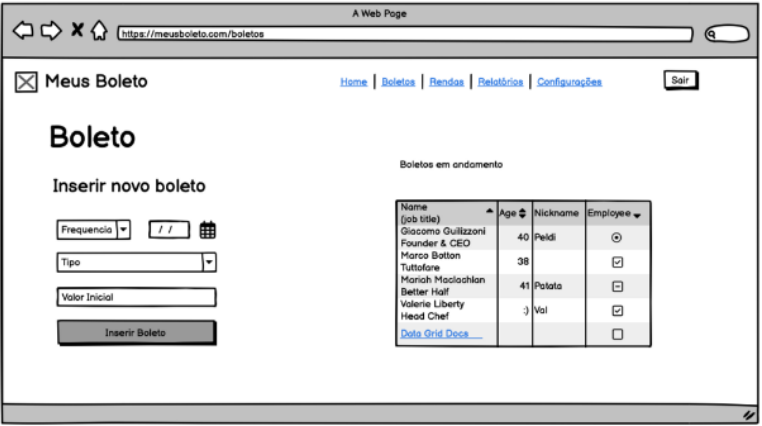
\includegraphics[scale=0.5]{images/CriarBoletoRenda.png}
	\end{center}
	\fonte{Autor (2024)}
\end{figure}


\textbf{CRITÉRIOS DE ACEITAÇÃO}

\begin{enumerate}
    \item Não deve inserir uma data válida;
    \item Deve permitir inserir um novo ‘boleto’ na base de dados para o
usuário;
    \item Deve inserir valores que não sejam números.
\end{enumerate}

\textbf{CRITÉRIOS DE ACEITAÇÃO - DETALHAMENTO}

\textbf{Critério de contexto (Válido como premissa para todos os critérios):}

\begin{itemize}
    \item[\textbf{Dado que}] entrei na aplicação
    \item[\textbf{E}] estou na tela para criacação de boletos
\end{itemize}


\begin{itemize}
    \item[] \textbf{1. Não deve inserir uma data válida;}

    \begin{itemize}
        \item[\textbf{Dado que}] preenchi o campo data com um valor invalido
        \item[\textbf{Quando}] pressiono o botão ``Inserir boleto''
        \item[\textbf{Então}] o sistema deve apresentar uma mensagem de erro avisando a incosistência (R3)
    \end{itemize}

    \item[] \textbf{2. Deve permitir inserir um novo ‘boleto’ na base de dados para o
usuário.}

    \begin{itemize}
        \item[\textbf{Dado que}] preenchi todos os campos corretamente
        \item[\textbf{Quando}] pressiono o botão ``Inserir Boleto''
        \item[\textbf{Então}] o sistema deve realizar a operação e informar o usuario
    \end{itemize}

    \item[] \textbf{3. Não deve permitir valores que não sejam números.}

    \begin{itemize}
        \item[\textbf{Dado que}] preenchi o campo 'Valor Inicial' com caracteres não números
        \item[\textbf{Quando}] pressiono o botão ``Inserir Boleto''
        \item[\textbf{Então}]  o sistema deve apresentar uma mensagem de erro avisando a incosistência (R3)
    \end{itemize}

    
\end{itemize}

\textbf{REGRAS DE NEGÓCIO DA HISTÓRIA:}

    R3 - Campos inconsistentes

    \begin{table}[htb]
        \caption{Tabela de inconsistências de inserir boletos}
        \centering
        \begin{tabular}{|c|c|}
        \hline
          \textbf{Incosistência}   &  \textbf{Mensagem} \\
        \hline
        Valor incorreto   & "O campo de valor somente aceita números!" \\
        \hline
        Data com caracteres inconsistêntes   & "verifique o campo de data!"  \\
        \hline
        \end{tabular}
        \fonte{Autor (2024)}
        \label{tab:tabela_login}
    \end{table}

\subsection{HU04 Deletar Boletos}

Sendo um usuário da aplicação, quero deletar item existente de despesa/renda para que eu exclua ele de minha dívidas/receitas.

\begin{figure}[htb]
	\caption{\label{fig:hu04}Página para deletar boletos.}
	\begin{center}
		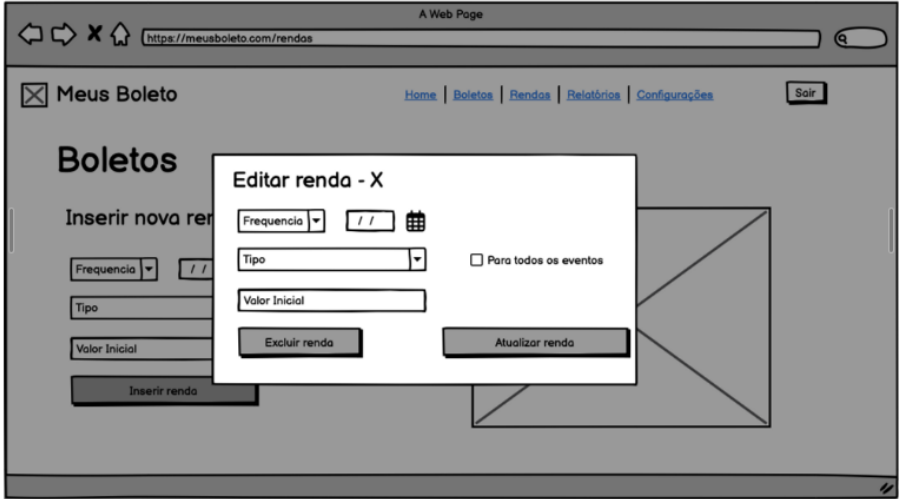
\includegraphics[scale=0.5]{images/EditarBoletoRenda.png}
	\end{center}
	\fonte{Autor (2024)}
\end{figure}

\textbf{CRITÉRIOS DE ACEITAÇÃO}

\begin{enumerate}
    \item Deve permitir o usuário excluir um boleto.
\end{enumerate}

\textbf{CRITÉRIOS DE ACEITAÇÃO - DETALHAMENTO}

\textbf{Critério de contexto (Válido como premissa para todos os critérios):}

\begin{itemize}
    \item[\textbf{Dado que}] entrei na aplicação
    \item[\textbf{E}] estou na tela para seleção de boleto
\end{itemize}


\begin{itemize}
    \item[] \textbf{1. Deve permitir o usuário excluir um boleto.}

    \begin{itemize}
        \item[\textbf{Dado que}] Selecionei um boleto para edição
        \item[\textbf{Quando}] pressiono o botão ``Excluir boleto''
        \item[\textbf{Então}] o sistema deve excluir a transação do sistema
    \end{itemize}
\end{itemize}

\subsection{HU05 Editar Boletos}

Sendo um usuário da aplicação, quero inserir um novo item de despesa/renda para que eu tenha um controle maior de minha dívidas/receitas.

\begin{figure}[htb]
	\caption{\label{fig:hu05}Página para editar boletos.}
	\begin{center}
		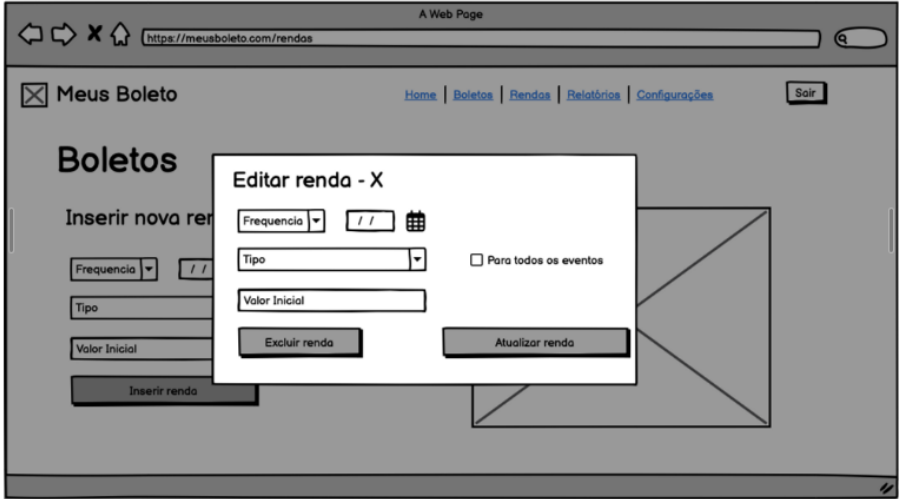
\includegraphics[scale=0.5]{images/EditarBoletoRenda.png}
	\end{center}
	\fonte{Autor (2024)}
\end{figure}


\textbf{CRITÉRIOS DE ACEITAÇÃO}

\begin{enumerate}
    \item Deve permitir a edição de um boleto.
\end{enumerate}

\textbf{CRITÉRIOS DE ACEITAÇÃO - DETALHAMENTO}

\textbf{Critério de contexto (Válido como premissa para todos os critérios):}

\begin{itemize}
    \item[\textbf{Dado que}] entrei na aplicação
    \item[\textbf{E}] estou na tela para seleção de boleto
\end{itemize}


\begin{itemize}
    \item[] \textbf{1. Deve permitir a edição de um boleto.}

    \begin{itemize}
        \item[\textbf{Dado que}] Selecionei um boleto para edição
        \item[\textbf{Quando}] clico em editar
        \item[\textbf{Então}] o sistema deve exibir o modal da figura \ref{fig:hu05} 
    \end{itemize}
\end{itemize}

\subsection{HU06 Criar fonte de Renda}

Sendo um usuário da aplicação, quero editar um item de despesa/renda para que eu consiga atualizar algum valor.

\begin{figure}[htb]
	\caption{\label{fig:hu06}Página para criar fonte de renda.}
	\begin{center}
		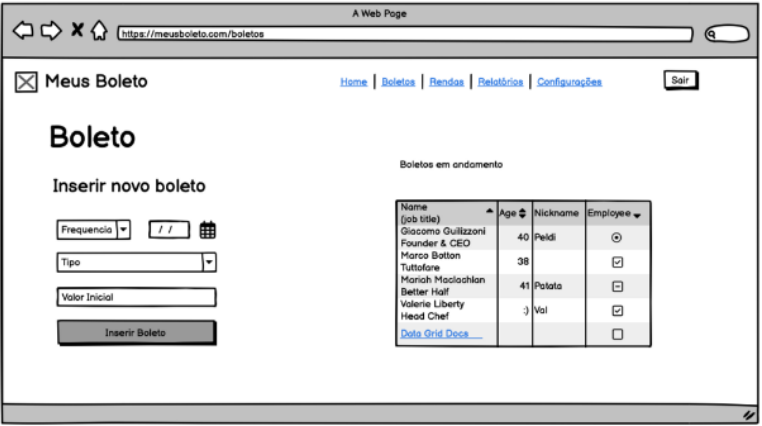
\includegraphics[scale=0.5]{images/CriarBoletoRenda.png}
	\end{center}
	\fonte{Autor (2024)}
\end{figure}

\textbf{CRITÉRIOS DE ACEITAÇÃO}

\begin{enumerate}
    \item Não deve inserir uma data válida;
    \item Deve permitir inserir uma nova ‘Renda’ na base de dados para o
usuário;
    \item Deve inserir valores que não sejam números.
\end{enumerate}

\textbf{CRITÉRIOS DE ACEITAÇÃO - DETALHAMENTO}

\textbf{Critério de contexto (Válido como premissa para todos os critérios):}

\begin{itemize}
    \item[\textbf{Dado que}] entrei na aplicação
    \item[\textbf{E}] estou na tela para criação de rendas
\end{itemize}


\begin{itemize}
    \item[] \textbf{1. Não deve inserir uma data válida;}

    \begin{itemize}
        \item[\textbf{Dado que}] preenchi o campo data com um valor invalido
        \item[\textbf{Quando}] pressiono o botão ``Inserir boleto''
        \item[\textbf{Então}] o sistema deve apresentar uma mensagem de erro avisando a incosistência (R4)
    \end{itemize}

    \item[] \textbf{2. Deve permitir inserir uma nova ‘Renda’ na base de dados para o
usuário.}

    \begin{itemize}
        \item[\textbf{Dado que}] preenchi todos os campos corretamente
        \item[\textbf{Quando}] pressiono o botão ``Inserir Renda''
        \item[\textbf{Então}] o sistema deve realizar a operação e informar o usuário (R4)
    \end{itemize}

    \item[] \textbf{3. Não deve permitir valores que não sejam números.}

    \begin{itemize}
        \item[\textbf{Dado que}] preenchi o campo 'Valor Inicial' com caracteres não números
        \item[\textbf{Quando}] pressiono o botão ``Inserir Boleto''
        \item[\textbf{Então}]  o sistema deve apresentar uma mensagem de erro avisando a inconsistência (R4)
    \end{itemize}

    
\end{itemize}

\textbf{REGRAS DE NEGÓCIO DA HISTÓRIA:}

    R4 - Campos inconsistentes

    \begin{table}[htb]
        \caption{Tabela de inconsistências de inserir rendas}
        \centering
        \begin{tabular}{|c|c|}
        \hline
          \textbf{Incosistência}   &  \textbf{Mensagem} \\
        \hline
        Valor incorreto   & "O campo de valor somente aceita números!" \\
        \hline
        Data com caracteres inconsistêntes   & "verifique o campo de data!"  \\
        \hline
        \end{tabular}
        \fonte{Autor (2024)}
        \label{tab:tabela_renda_inss }
    \end{table}


\subsection{HU07 Deletar fonte de Renda}

Sendo um usuário da aplicação, quero deletar um item de renda para que eu consiga excluir o item selecionado.

\begin{figure}[htb]
	\caption{\label{fig:hu07}Página para deletar fonte de renda.}
	\begin{center}
		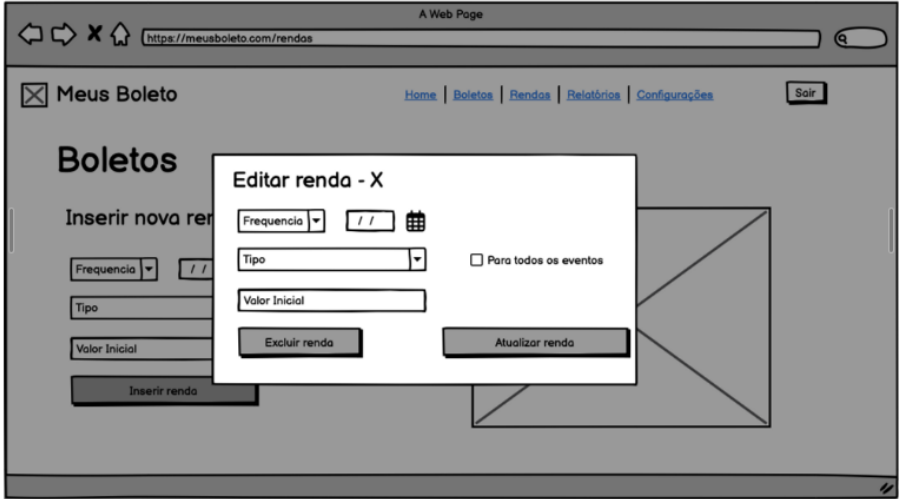
\includegraphics[scale=0.5]{images/EditarBoletoRenda.png}
	\end{center}
	\fonte{Autor (2024)}
\end{figure}

\textbf{CRITÉRIOS DE ACEITAÇÃO}

\begin{enumerate}
    \item Deve permitir o usuário excluir uma renda.
    
\end{enumerate}

\textbf{CRITÉRIOS DE ACEITAÇÃO - DETALHAMENTO}

\textbf{Critério de contexto (Válido como premissa para todos os critérios):}

\begin{itemize}
    \item[\textbf{Dado que}] entrei na aplicação
    \item[\textbf{E}] estou na tela para seleção de renda
\end{itemize}


\begin{itemize}
    \item[] \textbf{1. Deve permitir o usuário excluir uma fonte de renda.}

    \begin{itemize}
        \item[\textbf{Dado que}] Selecionei uma renda para edição
        \item[\textbf{Quando}] pressiono o botão ``Excluir Renda''
        \item[\textbf{Então}] o sistema deve excluir a transação do sistema
    \end{itemize}
\end{itemize}


\subsection{HU08 Editar fonte de Renda}

Sendo um usuário da aplicação, quero editar um item de renda para que eu consiga atualizar o item selecionado.

\begin{figure}[htb]
	\caption{\label{fig:hu07}Página para editar fonte de renda.}
	\begin{center}
		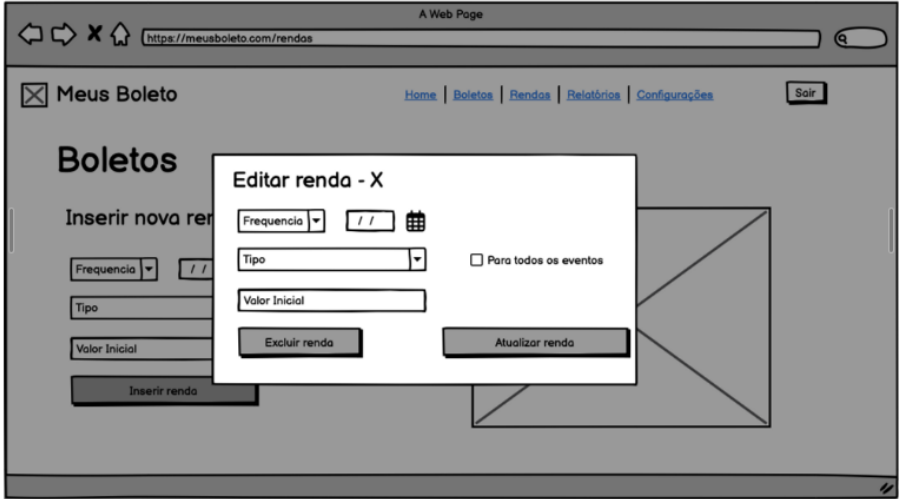
\includegraphics[scale=0.5]{images/EditarBoletoRenda.png}
	\end{center}
	\fonte{Autor (2024)}
\end{figure}

\textbf{CRITÉRIOS DE ACEITAÇÃO}

\begin{enumerate}
    \item Deve permitir a edição de uma renda.
\end{enumerate}

\textbf{CRITÉRIOS DE ACEITAÇÃO - DETALHAMENTO}

\textbf{Critério de contexto (Válido como premissa para todos os critérios):}

\begin{itemize}
    \item[\textbf{Dado que}] entrei na aplicação
    \item[\textbf{E}] estou na tela para seleção de renda
\end{itemize}


\begin{itemize}
    \item[] \textbf{1. Deve permitir a edição de uma renda.}

    \begin{itemize}
        \item[\textbf{Dado que}] Selecionei uma renda para edição
        \item[\textbf{Quando}] clico em editar
        \item[\textbf{Então}] o sistema deve exibir o modal da figura \ref{fig:hu07} 
    \end{itemize}
\end{itemize}

\subsection{HU12 Visualizar Resumo}

Sendo um usuário da aplicação, quero visualizar um resumo logo que entrar na aplicação para que eu veja os próximos vencimentos e créditos.

\begin{figure}[htb]
	\caption{\label{fig:Fig_1}Página inicial da aplicação.}
	\begin{center}
		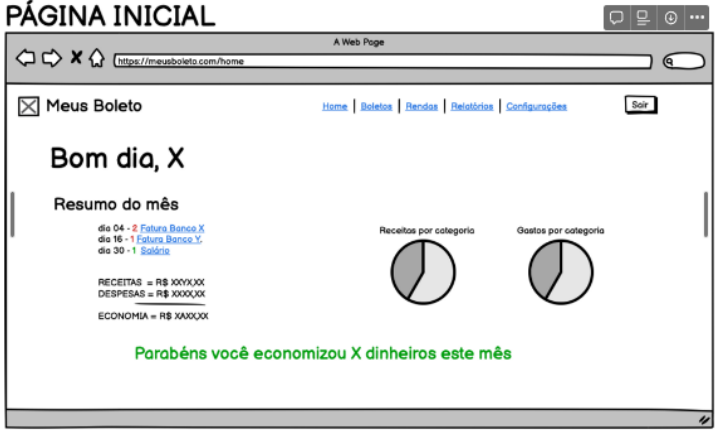
\includegraphics[scale=0.5]{images/TelaInicial.png}
	\end{center}
	\fonte{Autor (2024)}
\end{figure}

\textbf{CRITÉRIOS DE ACEITAÇÃO}

\begin{enumerate}
    \item Deve mostrar um gráfico resumindo as despesas do mês.
    \item Deve mostrar um resumo do saldo final.
\end{enumerate}

\textbf{CRITÉRIOS DE ACEITAÇÃO - DETALHAMENTO}

\textbf{Critério de contexto (Válido como premissa para todos os critérios):}

\begin{itemize}
    \item[\textbf{Dado que}] entrei na aplicação
    \item[\textbf{E}] estou na tela para seleção de renda
\end{itemize}


\begin{itemize}

      \item[] \textbf{1. Deve mostrar um gráfico resumindo as despesas do mês.}

    \begin{itemize}
        \item[\textbf{Dado que}] Estou na página inicial
        \item[\textbf{Então}] o sistema deve exibir o gráficos de resumo mensal de pr \ref{fig:hu07} 
    \end{itemize}

    \item[] \textbf{2. Deve mostrar um resumo do saldo final.}

    \begin{itemize}
        \item[\textbf{Dado que}]  Estou na página inicial
        \item[\textbf{Então}] o sistema deve exibir o resumo mensal das contas 
    \end{itemize}
    
\end{itemize}
% ---

% 5 - Diagrama de classes
%\phantompart
% ----------------------------------------------------------
\chapter{DIAGRAMA DE CLASSES}
% ----------------------------------------------------------

\begin{figure}[htb]
	\caption{\label{fig:classDiagram}Diagrama de classes.}
	\begin{center}
		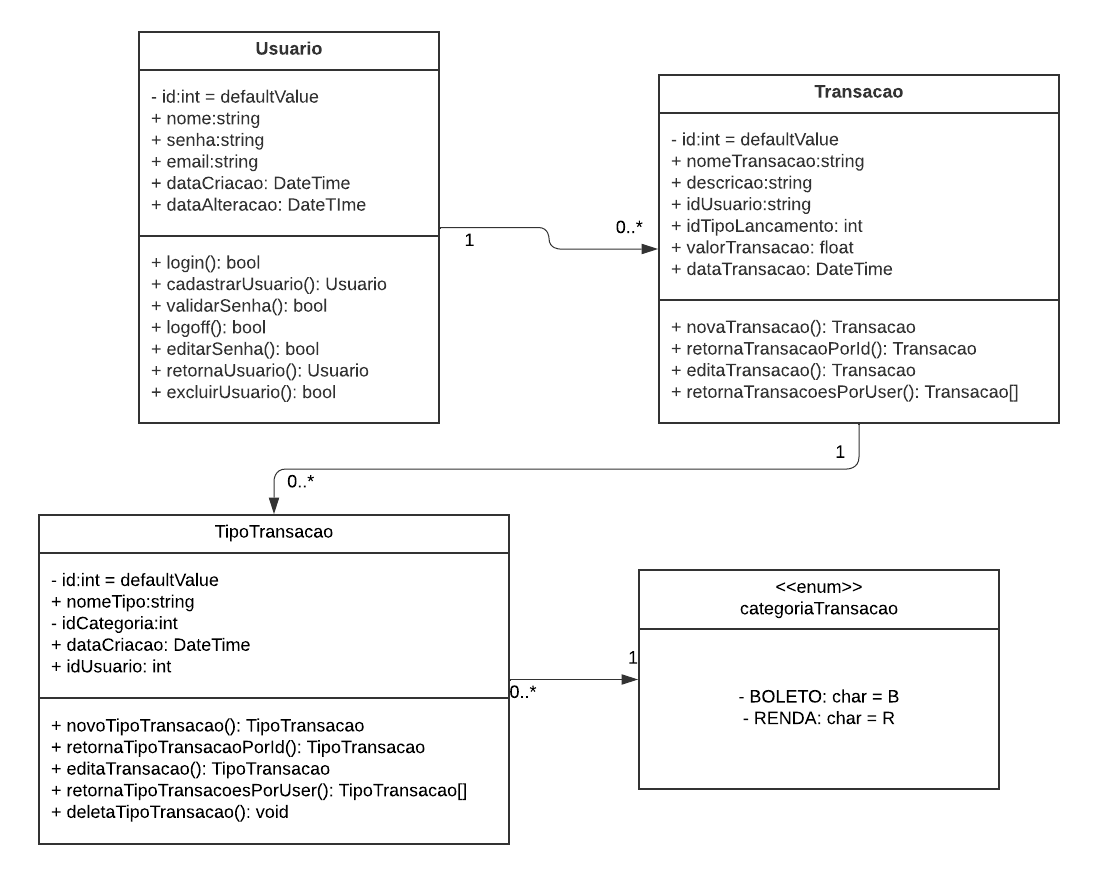
\includegraphics[scale=0.9]{images/classDiagram.png}
	\end{center}
	\fonte{Autor (2024)}
\end{figure}
% ---

% 6 - Diagrama de Sequência
%\phantompart
% ----------------------------------------------------------
%\chapter{Diagrama de sequência}
% ----------------------------------------------------------


% ---

% 7 - Diagrama Físico do banco de dados
%\phantompart
% ----------------------------------------------------------
\chapter{Diagrama físico do banco de dados}
% ----------------------------------------------------------

\begin{figure}[htb]
	\caption{\label{fig:db-diagram}Diagrama do banco de dados.}
	\begin{center}
		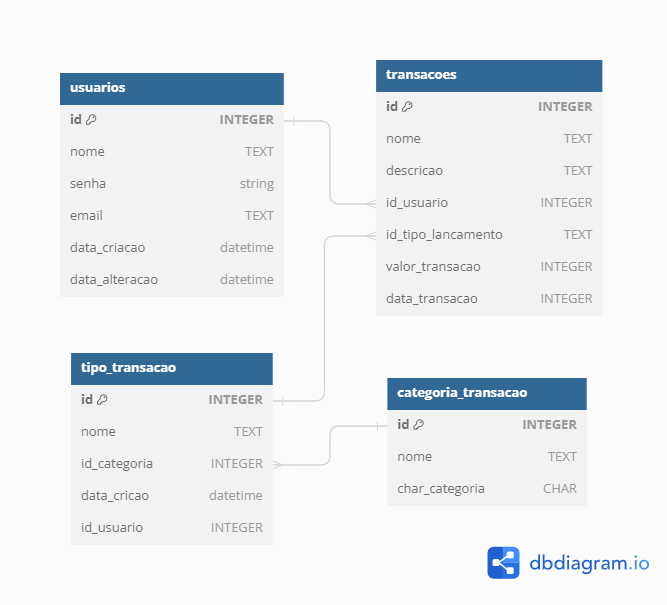
\includegraphics[scale=0.5]{images/db-diagram.png}
	\end{center}
	\fonte{Autor (2024)}
\end{figure}

% ---


% 9 - Diagrama de estados
%\phantompart
% ----------------------------------------------------------
%\chapter{Diagrama de estados}
% ----------------------------------------------------------

%\nocite{silva}
% ---

% ----------------------------------------------------------
% ELEMENTOS PÓS-TEXTUAIS
% ----------------------------------------------------------
\postextual
% ----------------------------------------------------------

% ----------------------------------------------------------
% Referências bibliográficas
% ----------------------------------------------------------
\begingroup
    \SingleSpacing\printbibliography[title=REFERÊNCIAS]
\endgroup

% ----------------------------------------------------------
% Glossário
% ----------------------------------------------------------
%
% Consulte o manual da classe abntex2 para orientações sobre o glossário.
%
%\glossary

% ----------------------------------------------------------
% Apêndices
% ----------------------------------------------------------

% ---
% Inicia os apêndices
% ---
%\begin{apendicesenv}
%	\partapendices* 
%	% ----------------------------------------------------------
\chapter{Descrição}
% ----------------------------------------------------------

Textos elaborados pelo autor, a fim de completar a sua argumentação. Deve ser precedido da palavra APÊNDICE, identificada por letras maiúsculas consecutivas, travessão e pelo respectivo título. Utilizam-se letras maiúsculas dobradas quando esgotadas as letras do alfabeto. 

\begin{quadro}[htb]
	\centering
	\caption{\label{qua:Quadro_2}Modelo A.}	
\begin{tabular}{|l|l|}
\hline
xxxx              & yyyyyyyyyyyyyyy    \\
\hline
xxxx              & yyyyyyyyyyyyyyy    \\
\hline
xxxx              & yyyyyyyyyyyyyyy    \\
\hline
xxxx              & yyyyyyyyyyyyyyy    \\
\hline
xxxx              & yyyyyyyyyyyyyyy    \\
\hline
xxxx              & yyyyyyyyyyyyyyy    \\
\hline
xxxx              & yyyyyyyyyyyyyyy    \\
\hline
rrrrrrrrrrrrrrrrr & eeeeeeeeeeeeeeeee  \\
\hline
xxxx              & yyyyyyyyyyyyyyy    \\
\hline
xxxx              & yyyyyyyyyyyyyyy    \\
\hline
rrrrrrrrrrrrrrrrr & eeeeeeeeeeeeeeeee  \\
\hline
xxxx              & yyyyyyyyyyyyyyy    \\
\hline
                  & ttttttttttttttttt  \\
\hline
rrrrrrrrrrrrrrrrr & eeeeeeeeeeeeeeeee  \\
\hline
ttttttttttttt     &                    \\
\hline
rrrrrrrrrrrrrrrrr & eeeeeeeeeeeeeeeee  \\
\hline
rrrrrrrrrrrrrrrrr & eeeeeeeeeeeeeeeee  \\
\hline
                  & gggggggggggggggggg \\
\hline
rrrrrrrrrrrrrrrrr & eeeeeeeeeeeeeeeee  \\
\hline
rrrrrrrrrrrrrrrrr & eeeeeeeeeeeeeeeee  \\
\hline
rrrrrrrrrrrrrrrrr & eeeeeeeeeeeeeeeee  \\
\hline
rrrrrrrrrrrrrrrrr & eeeeeeeeeeeeeeeee  \\
\hline
\end{tabular}
\fonte{Elaborada pelo autor (2016).}
\end{quadro}
%\end{apendicesenv}
% ---


% ----------------------------------------------------------
% Anexos
% ----------------------------------------------------------

% ---
% Inicia os anexos
% ---
%\begin{anexosenv}
%	\partanexos*
%	% ----------------------------------------------------------
\chapter{Descrição}
% ----------------------------------------------------------

São documentos não elaborados pelo autor que servem como fundamentação (mapas, leis, estatutos). Deve ser precedido da palavra ANEXO, identificada por letras maiúsculas consecutivas, travessão e pelo respectivo título. Utilizam-se letras maiúsculas dobradas quando esgotadas as letras do alfabeto. 

%\end{anexosenv}

%---------------------------------------------------------------------
% INDICE REMISSIVO
%---------------------------------------------------------------------
%\phantompart
%\printindex
%---------------------------------------------------------------------

\end{document}
